
\section{Usage Scenario}
\label{sec:scenario}

% We developed DataToon, a web-based tool for authoring data comics, based our design considerations.
To illustrate how \toolname{} accomplishes our goals and to describe key components of its interface, we describe the process taken by a hypothetical comic author named Aidan to create the comic in Figure~\ref{fig:comicbook}, adapted from Bach et al.~\cite{bach2016telling}. 

%on one appearing in the work of Bach et al. \cite{bach2016telling}.
%dynamic network dataset.
%Aiden is a high-school history teacher who wants to educate his students about the dynamics of European alliances preceding World War I. %He has experience with software like Excel and Tableau but no knowledge of graphic design software. To engage his students, he wants to use a data comic to communicate how the series of intricate alliances and conflicts evolved.
%Aidan, a high-school history teacher,  created a dataset representing a dynamic geographic and multi-faceted network where nodes are nations and links are alliances and oppositions that change over time. 



% It contains a list of European countries as nodes and alliances among the countries as links. Each alliance (i.e., link) has a temporal information about when it started and ended. 

Aidan opens \toolname{} in his web browser on a pen + touch-enabled device. The pen-tools menu (\autoref{fig:interface}A) represents the set of instruments his digital pen can acquire.  Aidan loads a dataset he previously created: a dynamic geographic and multi-faceted network containing countries and their alliances and oppositions over time. Dragging the file into the application instantiates both the legend panel and automatically generates a set of panels depicting notable structural patterns in the data (\autoref{fig:interface}C).  %Browsing legends and panels allows Aidan to recall the general content of his data. 

Aidan recalls that the evolution of alliances was interesting and he decides to explore these. He creates a new content panel by dragging the {\it Country} node type from the legend panel onto the canvas. Using the time slider for these panels (\autoref{fig:teaser}B), he filters 
\includegraphics[scale=0.02]{figures/filter_pen.png} the data back and forth to explore how the alliances changed over time. He duplicates panels as he finds interesting times, jotting down notes on them using the pencil 
\includegraphics[scale=0.02]{figures/draw_pen.png} (\autoref{fig:teaser}D).

%  he refine his ideas about the story to tell to his students. For example,

Continuing this process of exploration, Aidan now has multiple panels with annotated insights. He proceeds to craft a story for his comic by organizing them on the canvas. He wants to start with an overview of the nations involved, so he drops an image file containing a map of Europe (\autoref{fig:interface}G) into a panel, adjusting the location of each node with the \textit{Layout} pen 
\includegraphics[scale=0.02]{figures/layout_pen.png} (\autoref{fig:interface}H). He extracts country names from the data to place them on the map with the \textit{Label} pen 
\includegraphics[scale=0.02]{figures/label_pen.png}. 
%Finally, he adds a caption inside the panel to set the initial tone of the story (\autoref{fig:teaser}F).

% Once he has some idea about the narrative, he begins creating a comic strip. To show the countries in a geographic context, he loads an image showing the map of Europe (\autoref{fig:workflow}b). He wants to start by showing all the countries on the map. He uses the image as a background of the panel and positions each country node in its geographic location using the \textit{Control} pen (
\includegraphics[scale=0.05]{figures/control_pen.png}). He also creates labels to reveal the names of the countries using the \textit{Annotation} pen (
\includegraphics[scale=0.05]{figures/annotation_pen.png}). Finally, he creates a caption inside the panel to set the initial tone of the story (\autoref{fig:workflow}c).


% collecting, arranging, piling panels that may be interesting to include in the comic.

% Load image. and layout nodes in the gegraph


% He realizes the size of the panel is too small to show all the nodes, thus stretches it by dragging its right border to further right. 

After establishing the context of the story, Aidan wants to show the evolution of alliances in Europe. He reuses panels that he created earlier, transforming his rapid handwritten annotations into visual clusters around nodes, captions and labels. While he pans and zooms his first panel to emphasize two nodes (\autoref{fig:interface}J), he realizes that the difference between this panel and the first one may be too great and that his audience may fail to see the connection. He acquires the \textit{Magic} pen 
\includegraphics[scale=0.05]{figures/annotation_pen.png} to interpolate between these panels and generate intermediary ones (\autoref{fig:teaser}G). 

He generates a time caption for the last panel by dragging  the time label from the slider (\autoref{fig:interface}K, left). Duplicating this panel (\autoref{fig:interface}I) and adjusting the time automatically updates the caption (\autoref{fig:interface}K, right). Uncertain about what to show next, Aidan uses the \textit{Magic} pen 
\includegraphics[scale=0.05]{figures/annotation_pen.png} to trigger suggested panels with interesting patterns  (\autoref{fig:teaser}C). 



% He duplicates the first panel and adds the link type of \textit{Alliance} (\autoref{fig:workflow}d). He adjusts the time slider to 1839, to begin with, showing the neutrality contract % neutrality violation contract
% between the United Kingdom and Belgium. He double-taps the slider to create a caption using the current time as its text (\autoref{fig:workflow}e). 

% He lassos the two nodes to highlight, which make the rest of the countries muted into the background (\autoref{fig:workflow}f, 
\includegraphics[scale=0.05]{figures/annotation_pen.png}).

% Switching to the \textit{Control} pen (
\includegraphics[scale=0.05]{figures/control_pen.png}), he pans and zooms to set the focus of the panel to the two nodes.

As his comic nears completion, he customizes the node and link representations. For instance, he  draws a custom sketchy representation for all nodes (\autoref{fig:interface}D). To emphasize France among all countries, he paints its flag (\autoref{fig:teaser}E).
%to emphasizes the isolation of France due to the alliances of surrounding countries, he invokes the secondary canvas for the France node and
 This custom node representation is automatically propagated to all panels.  %\matt{R2's comment on the restrictiveness of data binding addresses this part of the scenario, but here is probably not the best place to discuss it} 
 Satisfied with his comic, he exports the comic as an image that he can share with his students.

% Now he wants to explain the Three Emperors alliance between Germany, Russia and Austria, which began in 1873. He again starts by duplicating the previous panel, which copies everything including the caption as well as underlying data bindings. Once he set the year to 1873 in the new panel, the time caption is automatically updated (\autoref{fig:workflow}g left). He now zooms into the three countries and highlights them into the foreground. To show the significance of the alliance, he adds a colored background to the three nodes, using the \textit{Annotation} pen but now with the pen button pressed (\autoref{fig:workflow}h).



% 
\includegraphics[scale=0.05]{figures/pencil.png}). He likes the freedom of creating his own unique style. He draws a custom, comic-like, sketchy appearance for each node by invoking a contextualized canvas from the legend panel (\autoref{fig:workflow}i). He similarly draws a country flag for France by lassoing its node using \textit{Pencil} (
\includegraphics[scale=0.05]{figures/pencil.png}) with the pen button pressed. These custom visuals are automatically propagated to all other panels. Before finishing, he saves the current comic strip as an image to see if it looks good in print.



% He create a series of panels and jot down a node on each panel on what to show 



% 1. Top-down 

% starting with story boarding. create empty panels, layout them, write down notes, etc.

% 2. Bottom up

% create a detailed panel, copy and paste progressively.





% \begin{figure*}[!t]
%     \centering
% 	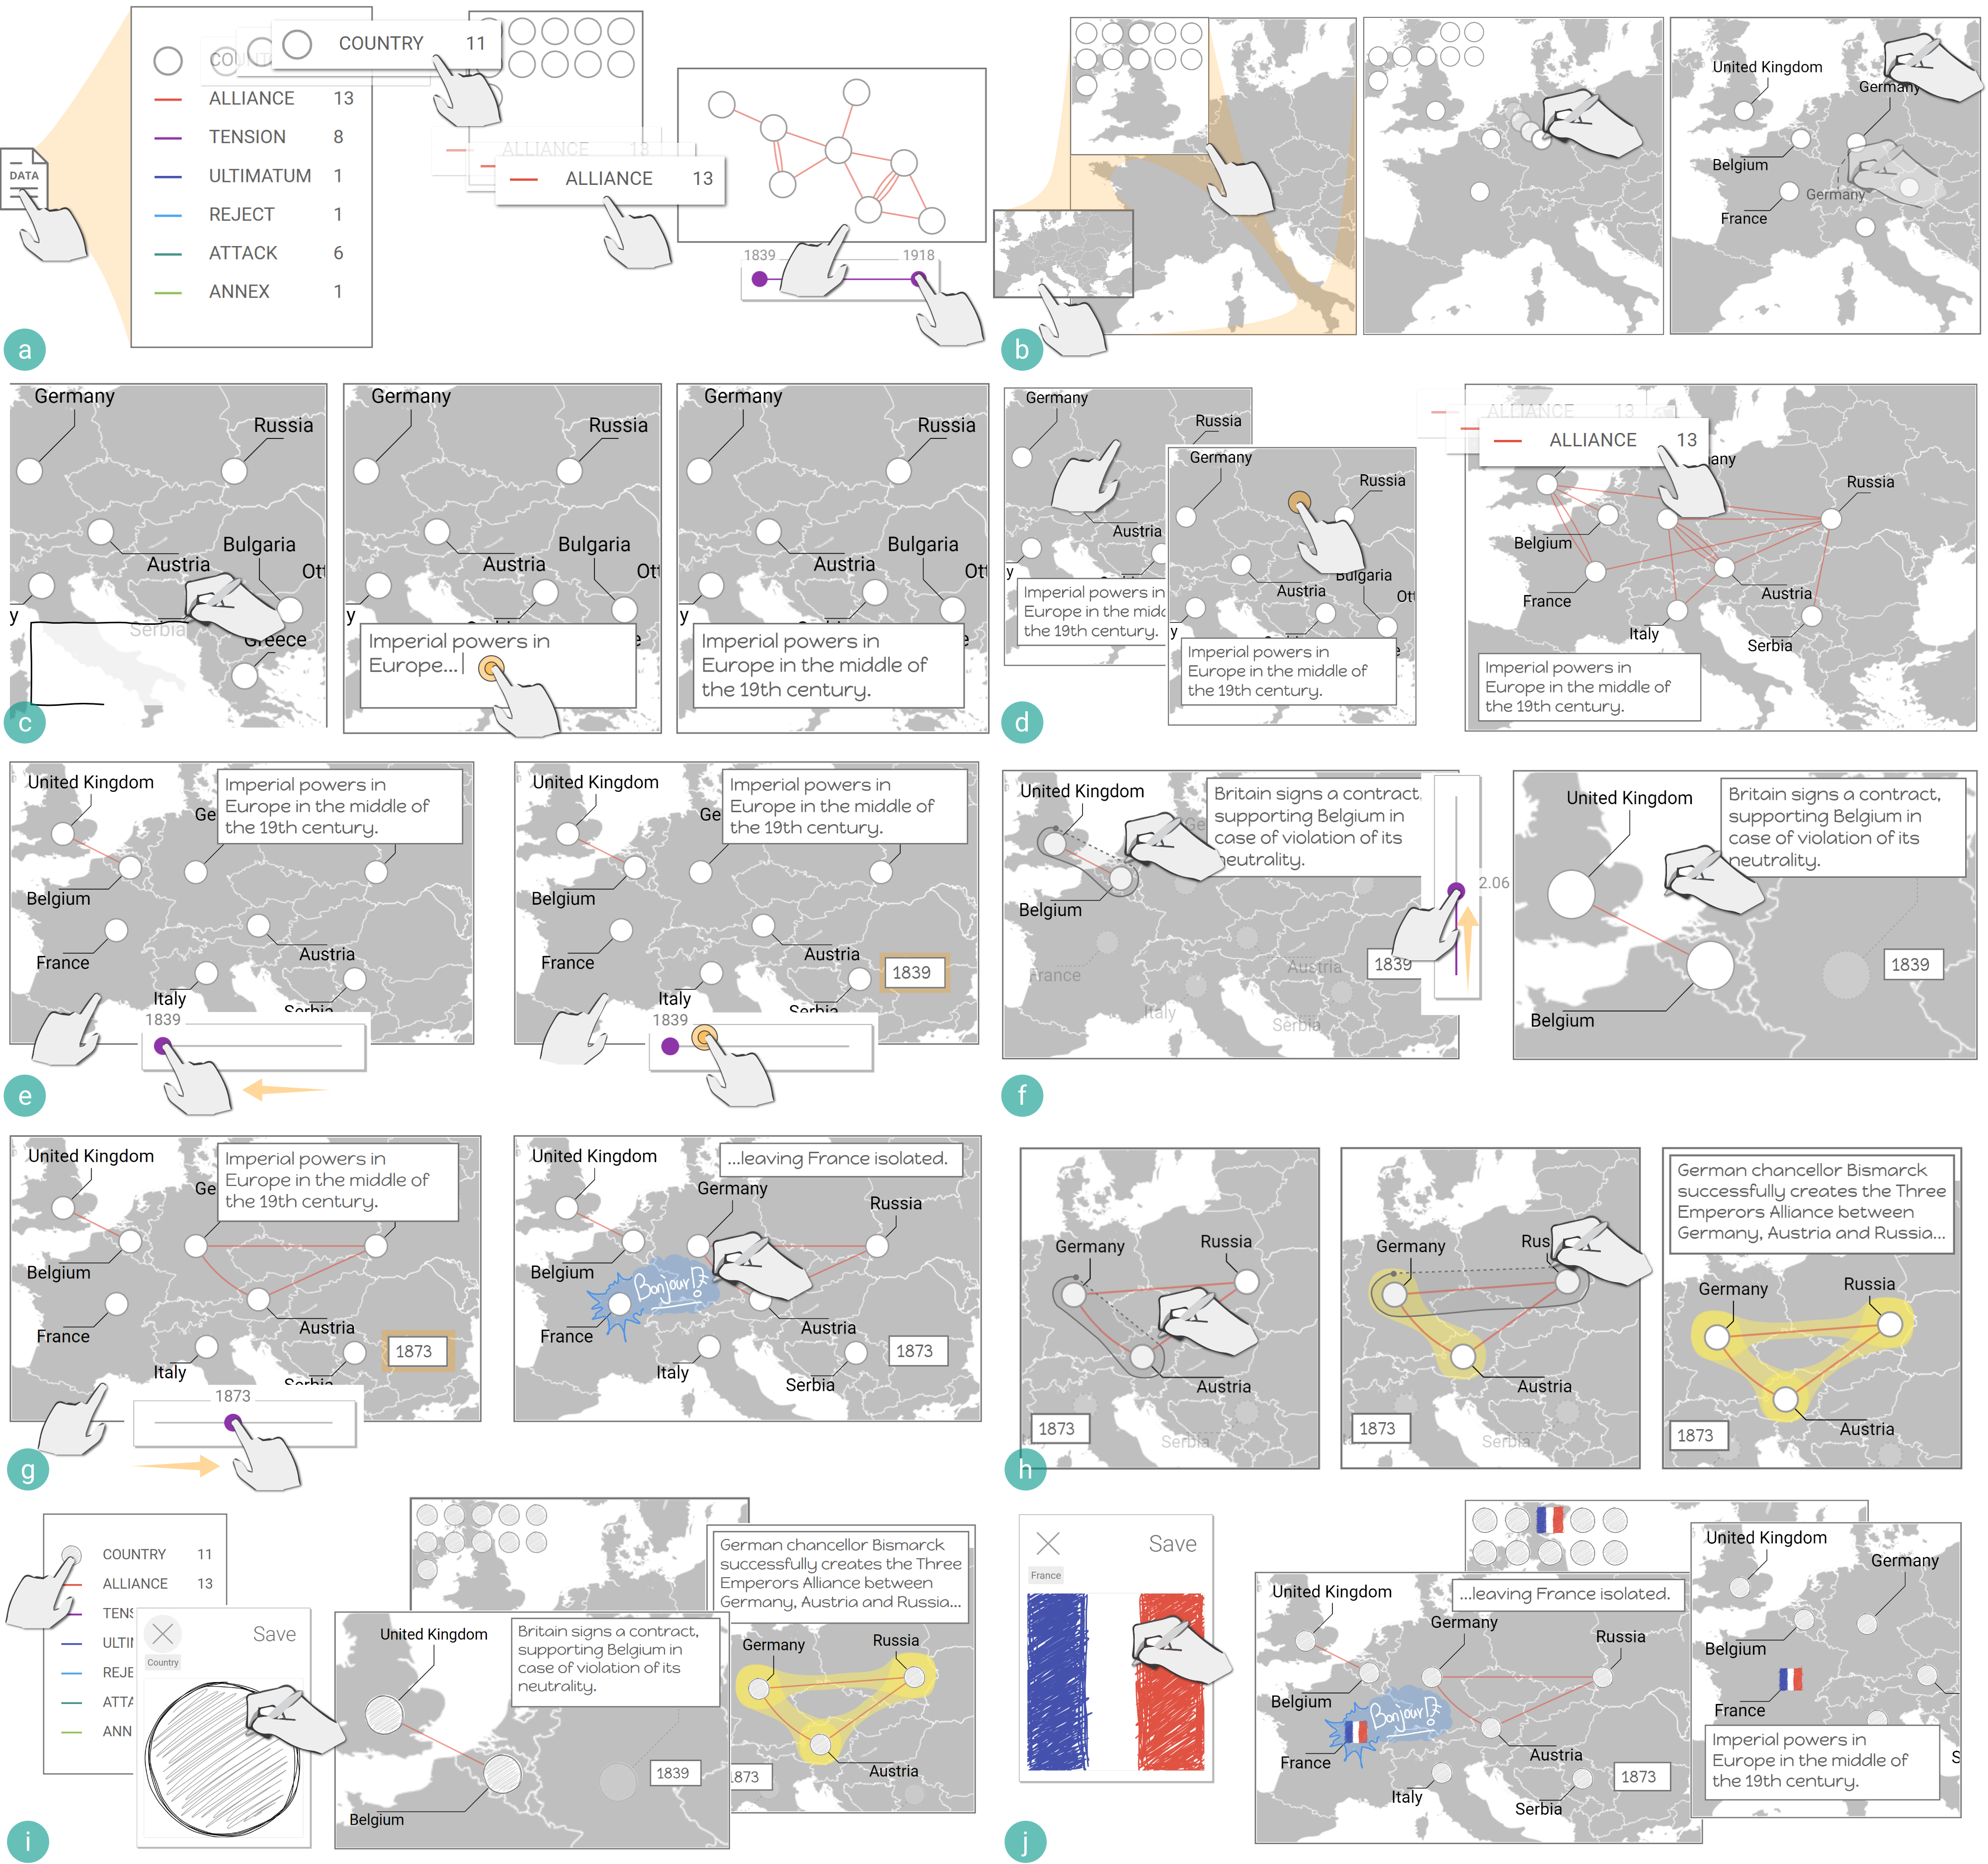
\includegraphics[width=\textwidth]{figures/workflow_full} 
% 	\caption{The workflow of creating the data comic described in \autoref{sec:workflow} and shown in \autoref{fig:tool_overview}. (a) importing a dataset to create the legend panel and fluidly exploring the data through simple drag and drop and the time slider. (b) importing a background image, laying out nodes, and creating labels. (c) creating a caption by drawing a rectangle and double-tapping it to edit its text. (d) duplicating the panel through hold and tap, and incrementally adding additional data to the panel. (e) filtering data using the time slider and creating a time caption by double-tapping it. (f) lassoing nodes to show in the foreground and panning and zooming through the combination of pen and touch. (g) updating the time caption automatically and adding a freeform annotation through sketching. (h) Creating a highlighted group. (i) the contextual canvas allows the author to sketch new visual mappings for all country nodes and for (j) France specifically.}
%     \vspace{-0.2cm}
%     % \caption{\rev{Five} examples of data comics created using \toolname{}}
%     \label{fig:workflow}
% \end{figure*}

% \begin{figure*}[!t]
% 	\subfigure[]
% 	{
% 	   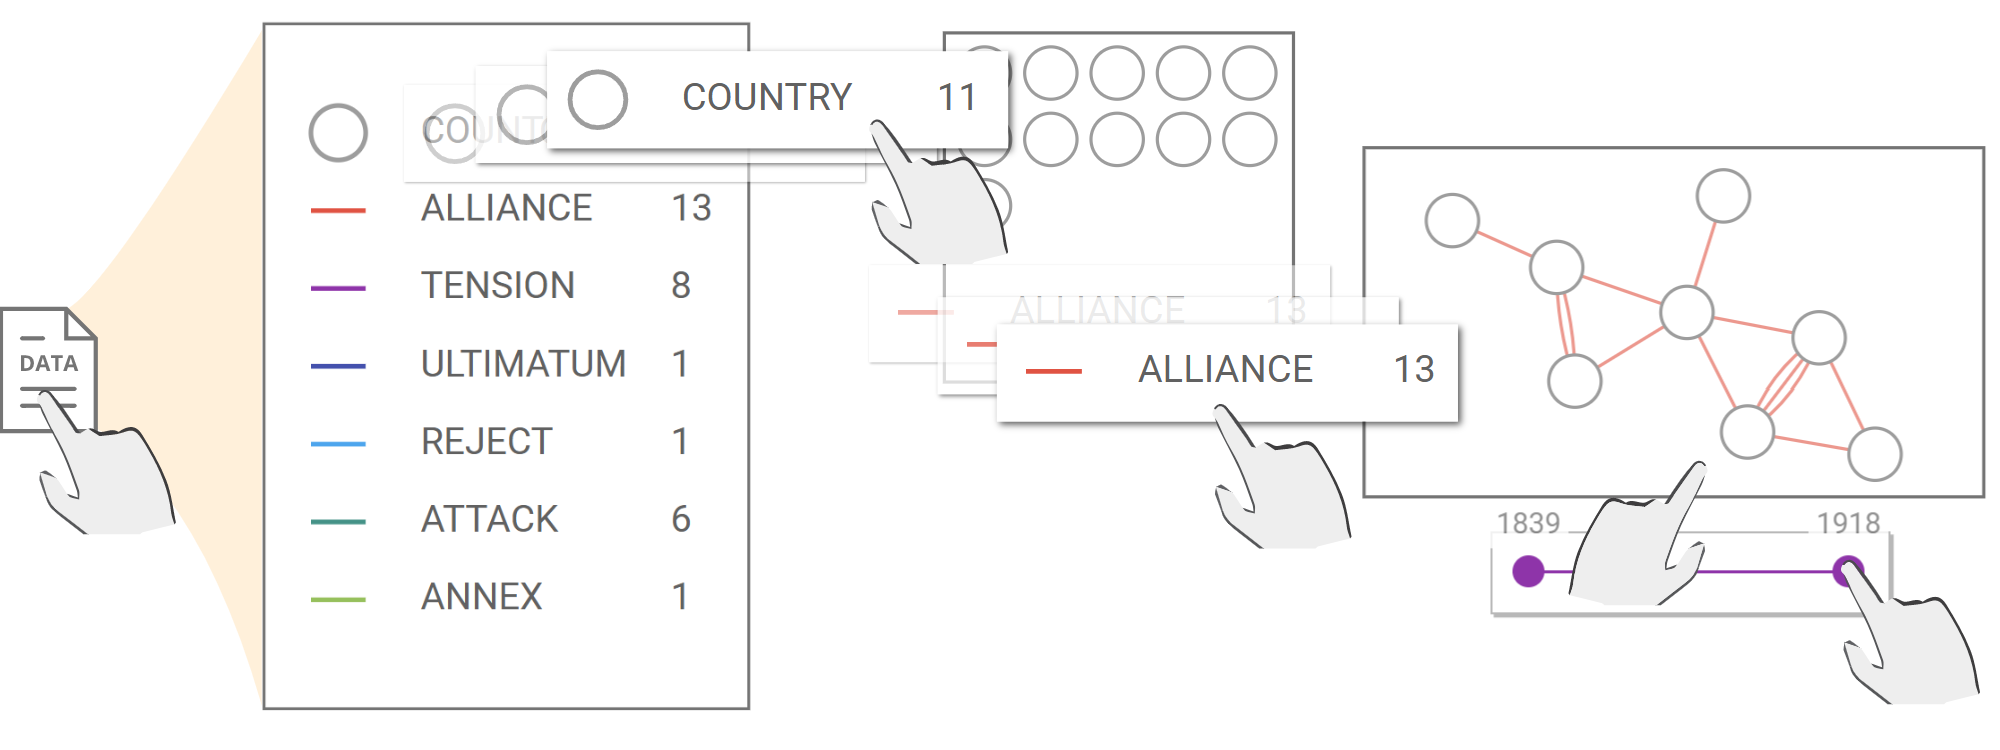
\includegraphics[width=1\columnwidth]{figures/workflow1}
% 		\label{fig:workflow1}
% 	}
% 	\hfill
% 	\subfigure[]
% 	{
% 	   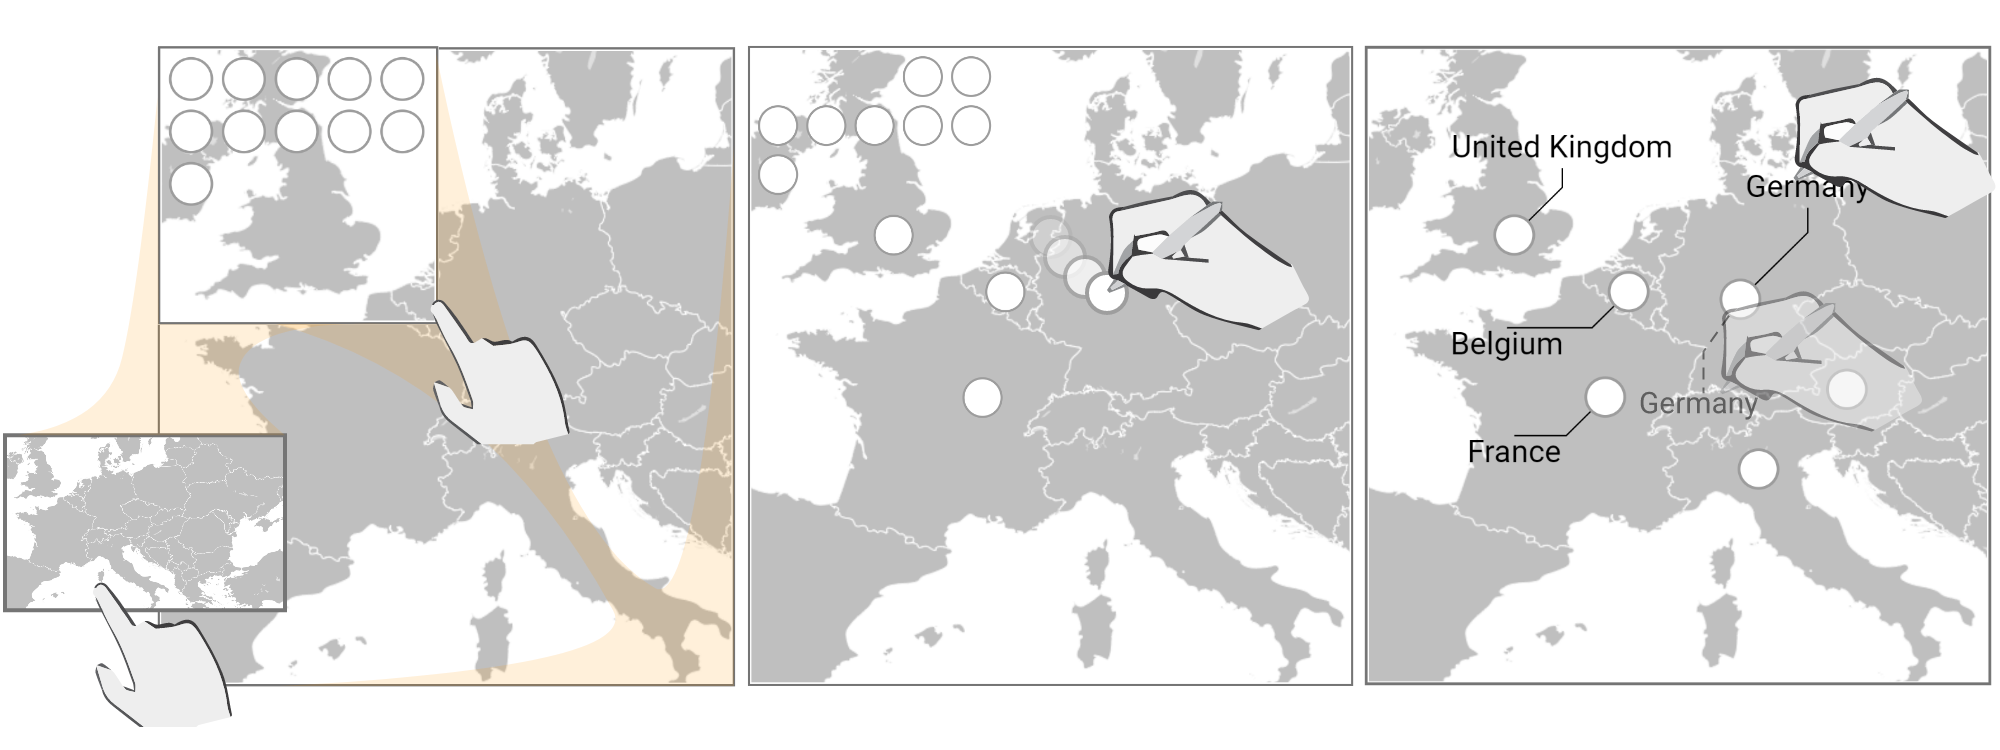
\includegraphics[width=1\columnwidth]{figures/workflow2}
% 		\label{fig:workflow2}
% 	}
% 	\hfill
% 	\subfigure[]
% 	{
% 		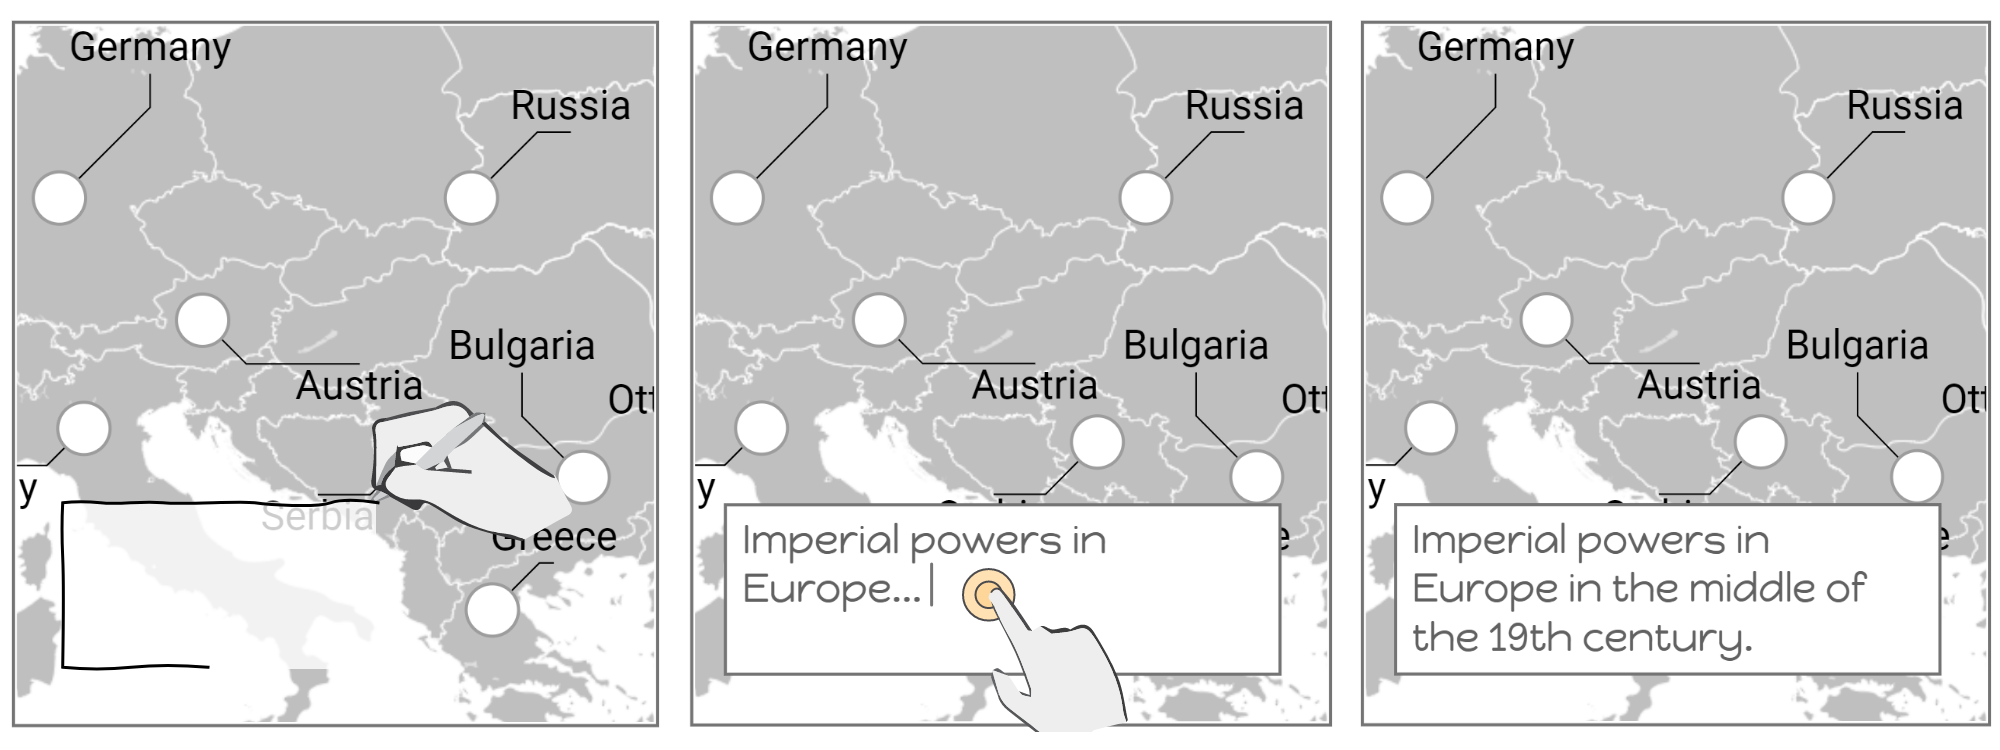
\includegraphics[width=1\columnwidth]{figures/workflow3}
% 	   \label{fig:workflow3}
% 	}
% 	\hfill
% 	\subfigure[]
% 	{
% 	   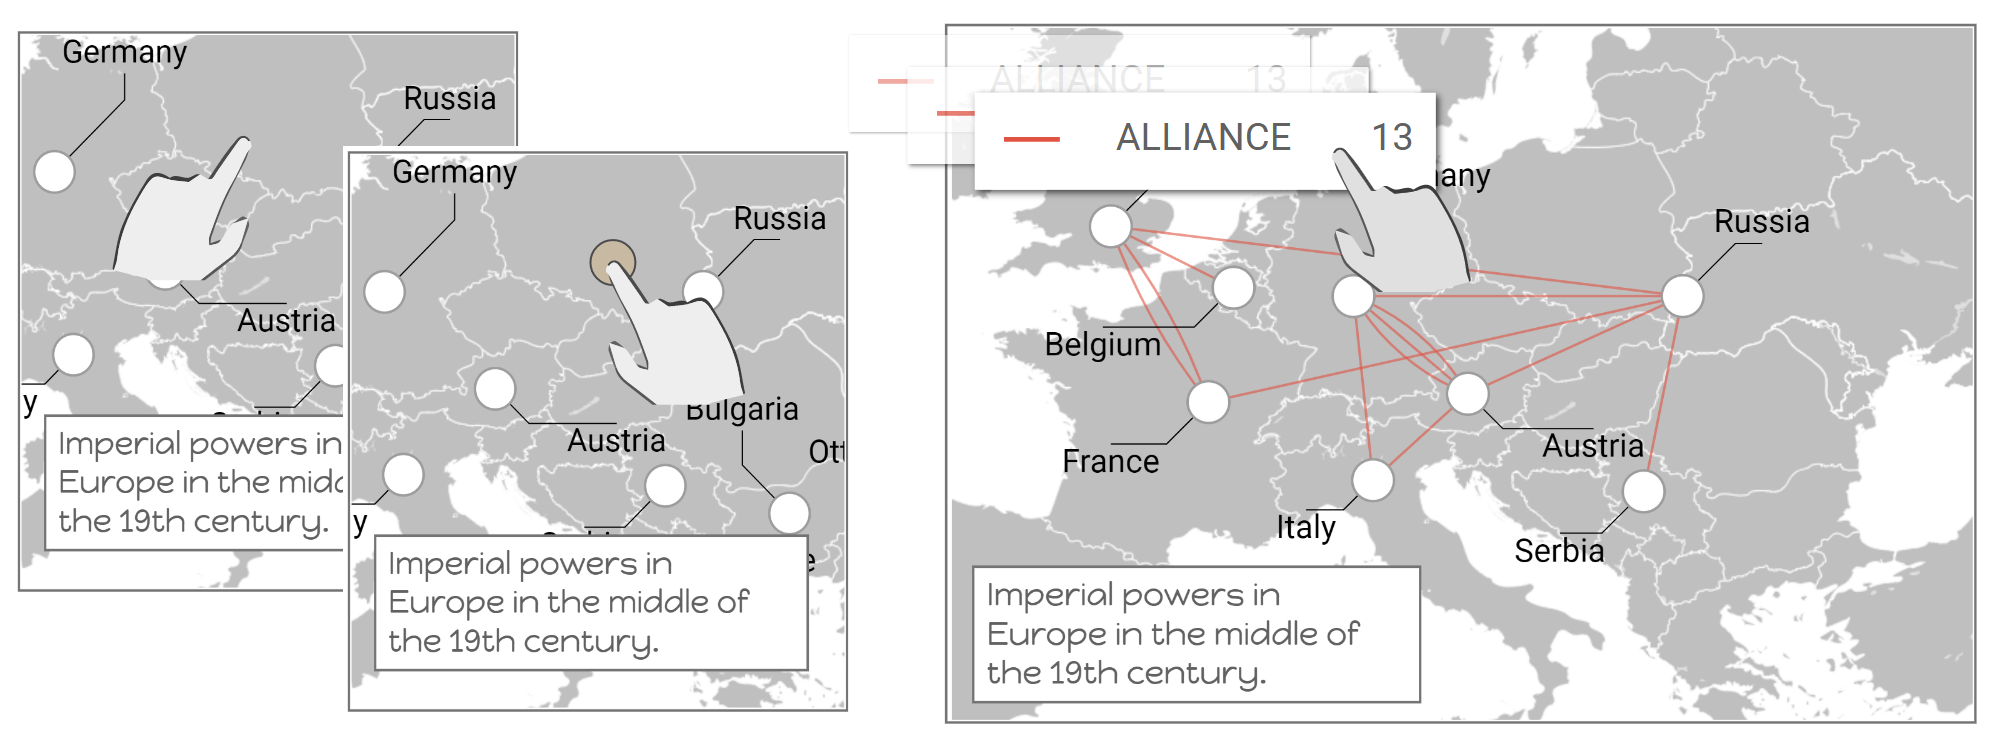
\includegraphics[width=1\columnwidth]{figures/workflow4}
% 		\label{fig:workflow4}
% 	}
% 	\hfill
% 	\subfigure[]
% 	{
% 		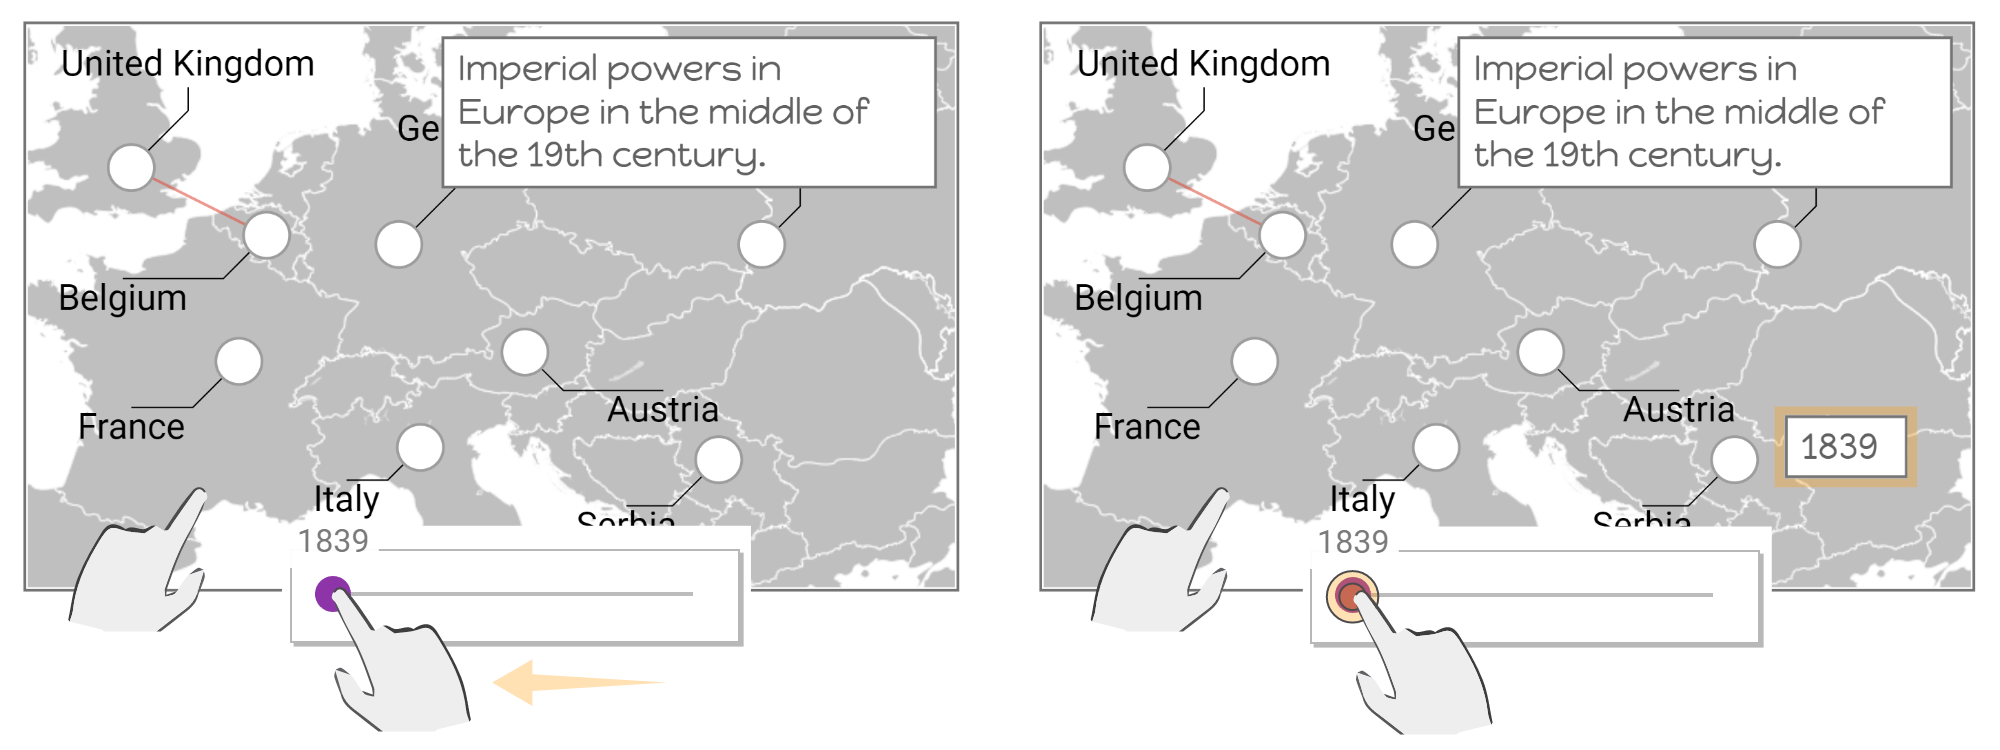
\includegraphics[width=1\columnwidth]{figures/workflow5}
% 		\label{fig:workflow5}
% 	}
% 	\hfill
% 	\subfigure[]
% 	{
% 		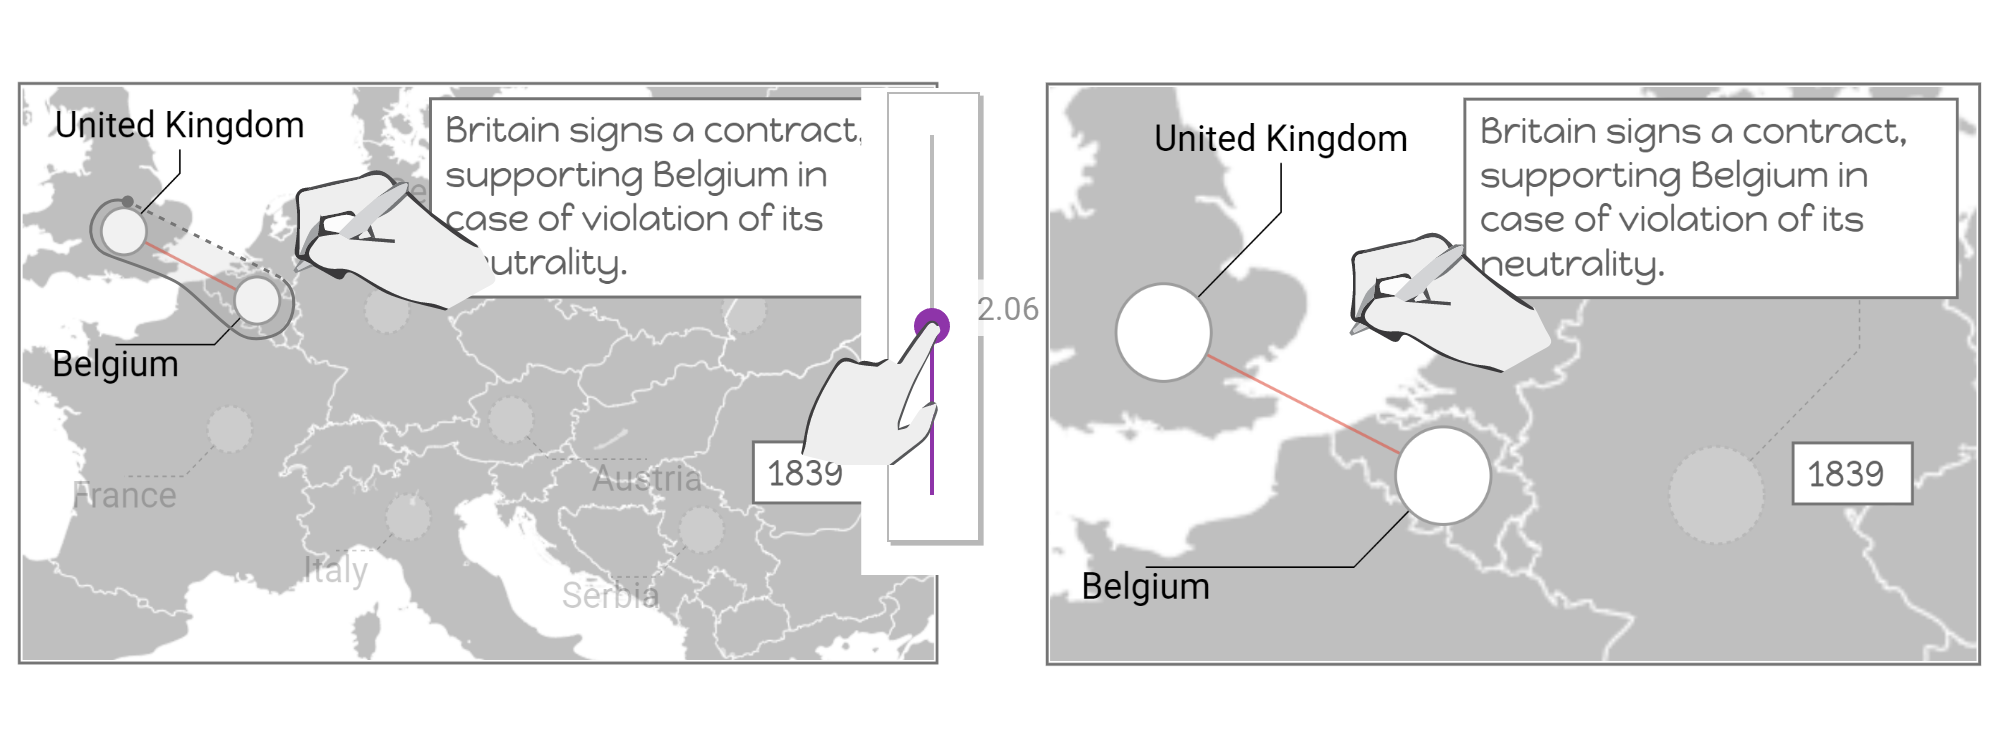
\includegraphics[width=1\columnwidth]{figures/workflow6}
% 		\label{fig:workflow6}
% 	}
% 	\hfill
% 	\subfigure[]
% 	{
% 		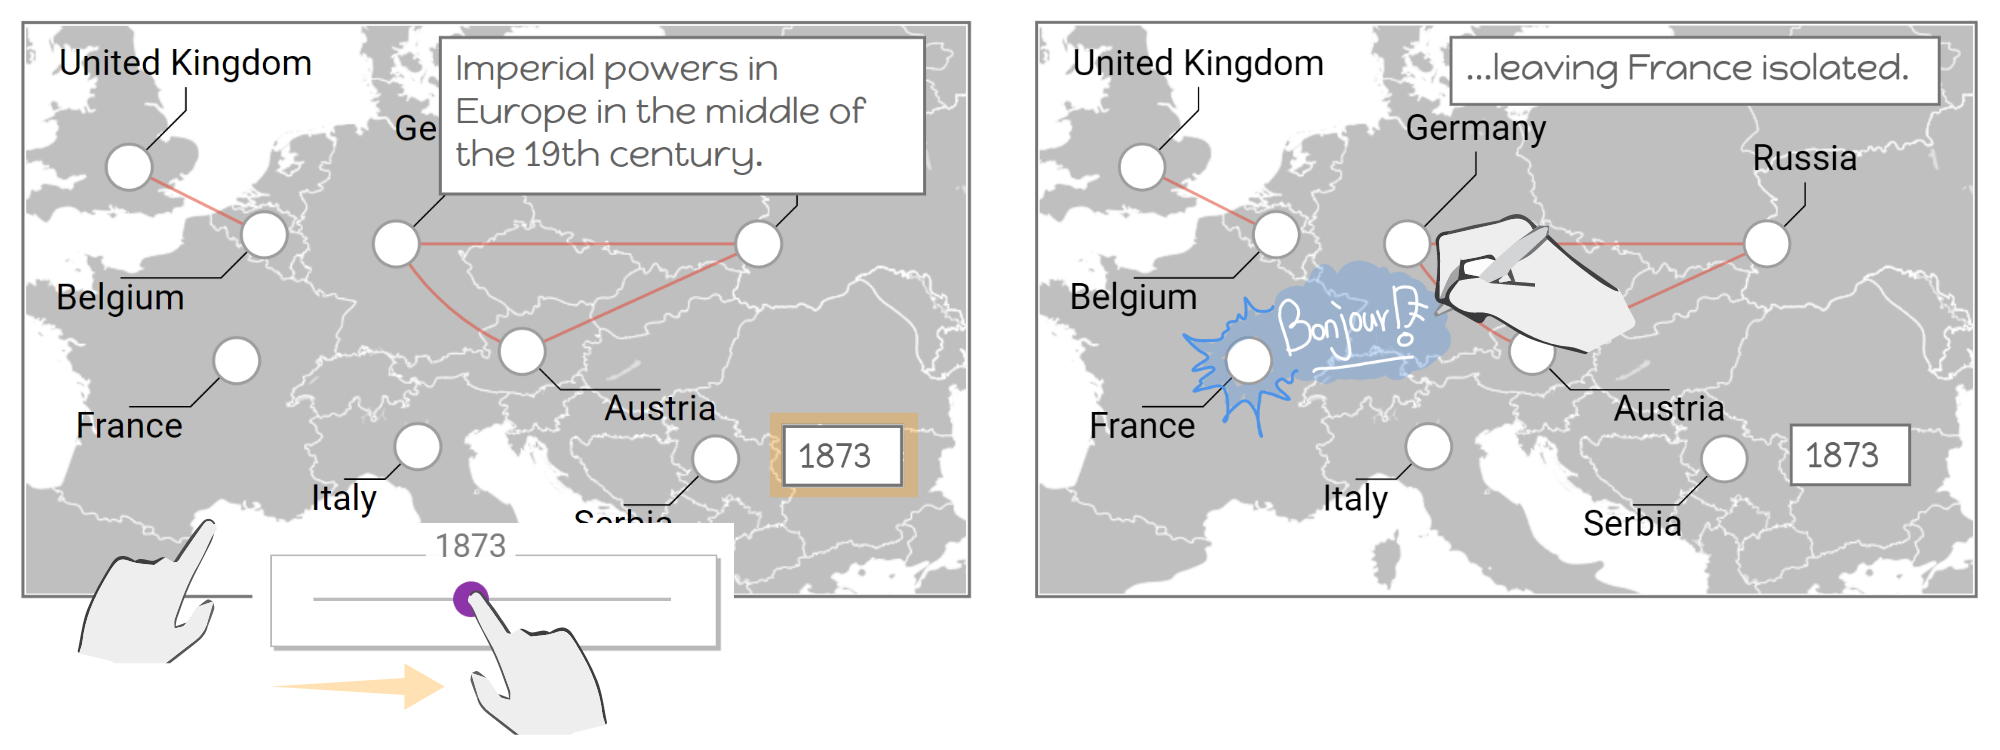
\includegraphics[width=1\columnwidth]{figures/workflow7}
% 		\label{fig:workflow7}
% 	}
% 	\hfill
% 	\subfigure[]
% 	{
% 		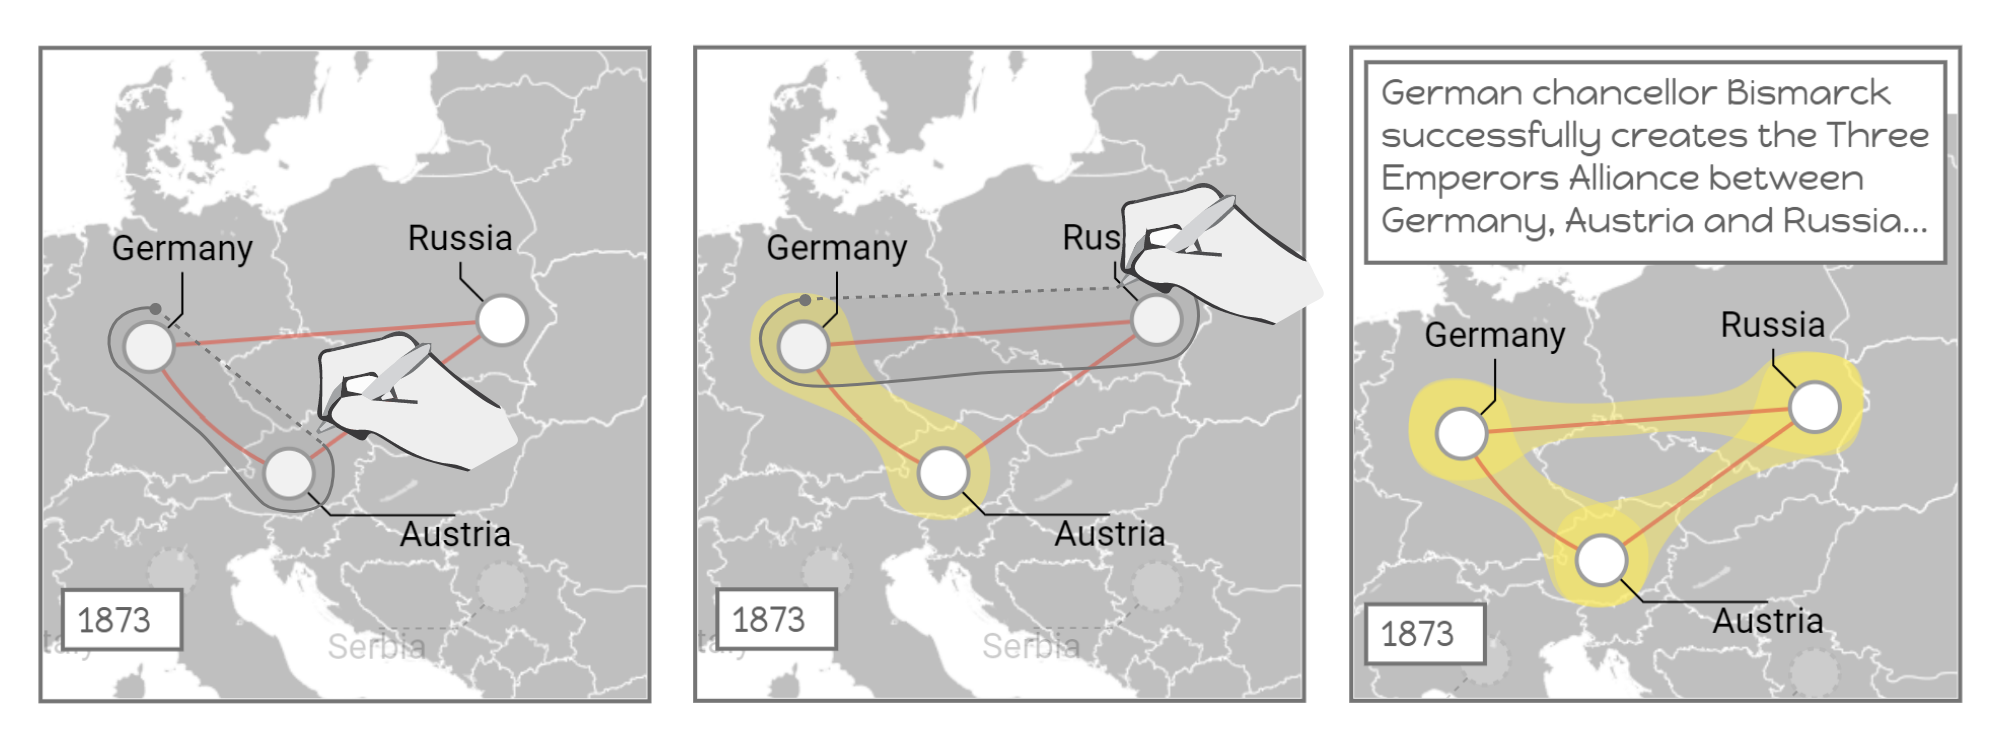
\includegraphics[width=1\columnwidth]{figures/workflow8}
% 		\label{fig:workflow8}
% 	}
% 	\hfill
% 	\subfigure[]
% 	{
% 		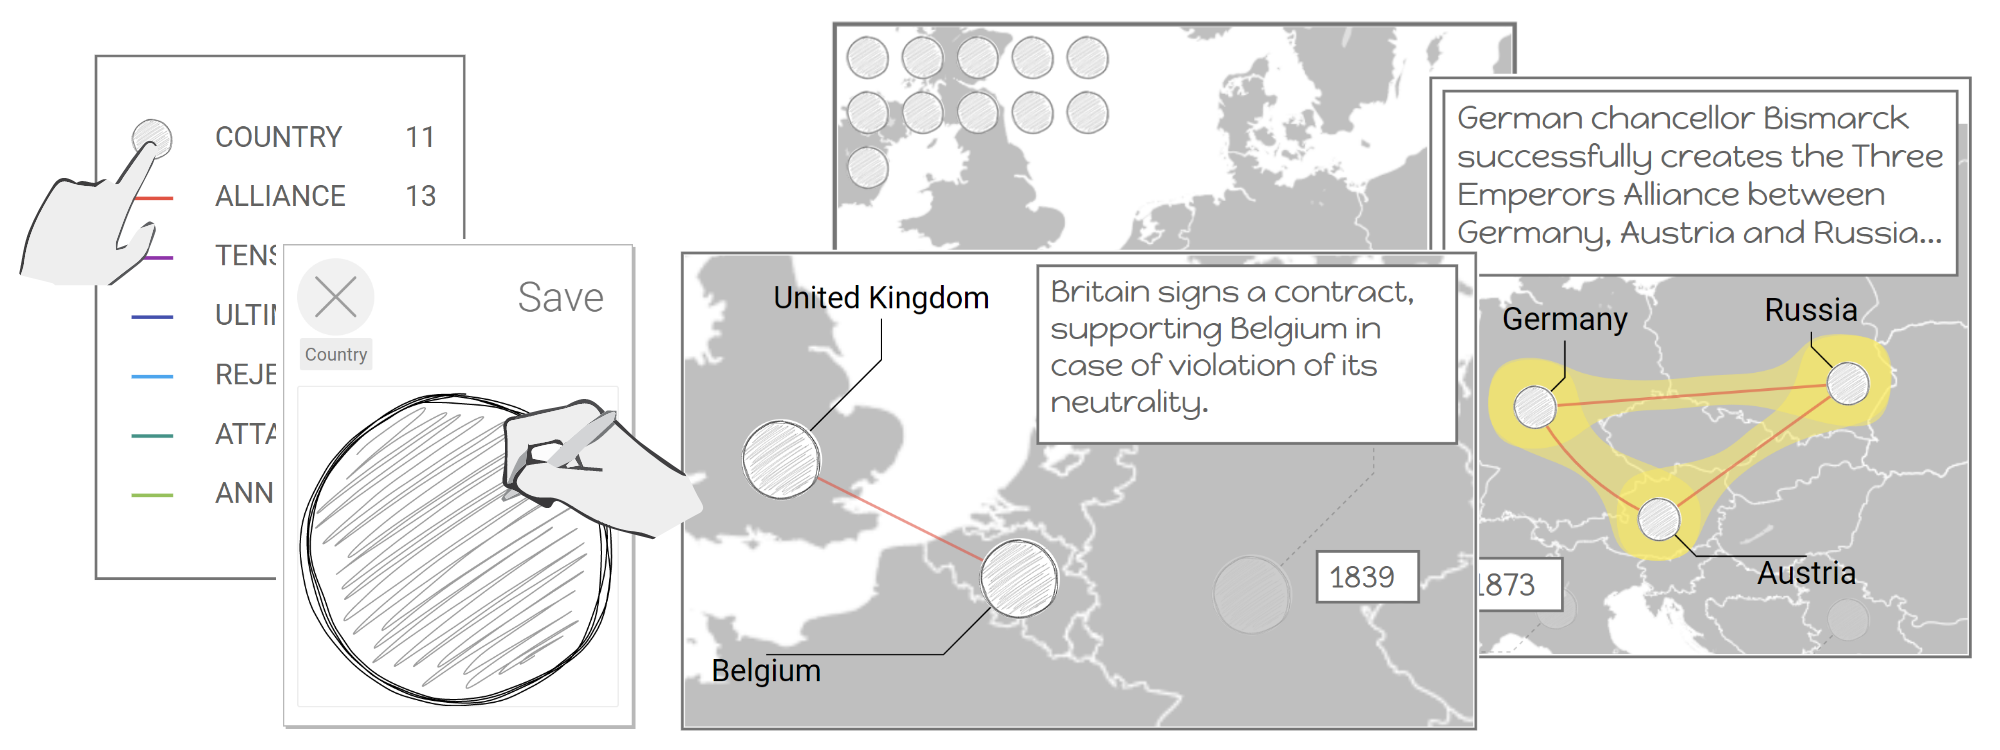
\includegraphics[width=1\columnwidth]{figures/workflow9}
% 		\label{fig:workflow9}
% 	}
% 	\hfill
% 	\subfigure[]
% 	{
% 		\includegraphics[width=1\columnwidth]{figures/workflow10}
% 		\label{fig:workflow10}
% 	}
%    \caption{The workflow of creating the data comic described in \autoref{sec:workflow} and shown in \autoref{fig:tool_overview}. (a) Importing a dataset to create the legend panel and fluidly exploring the data through simple drag and drop and the time slider. (b) Importing a background image, laying out nodes, and creating labels. (c) creating a caption by drawing a rectangle and double-tapping it to edit its text. (d) Duplicating the panel through hold and tap, and incrementally adding additional data to the panel. (e) Filtering data using the time slider and creating a time caption by doube-tapping it. (f) Lassoing nodes to show in the foreground and panning and zooming through the combination of pen and touch. (g) Updating the time caption automatically and adding a freeform annotation through sketching. (h) Creating a highlighted group. (i) Updating a visual mapping for all country nodes. (j) Updating a visual mapping for France. }
%    \label{fig:workflow}
%    \end{figure*}
